\chapter{Theoretical Background}

\label{chap:ch2}
\section{Natural Language Processing}

\quad This section explores Natural Language Processing (NLP), an important area in artificial intelligence that focuses on how computers understand and work with human language. NLP combines language studies with machine learning techniques to help machines understand, interpret, and generate human language in a useful way.

The basics of NLP are built on various tasks that address different parts of language processing. These tasks range from simple text handling to more complex activities like translating languages, analyzing emotions in text, and identifying important entities such as names and dates. By looking at these common NLP tasks, this section aims to provide an overview of the most common methods and algorithms that enable machines to process natural language.

\textbf{Tokenization} is the process of splitting text into individual words or tokens. This is a fundamental step for many NLP tasks, as it breaks down the text into manageable pieces that can be analyzed separately. Proper tokenization is crucial because it directly affects the performance of subsequent NLP processes. Challenges in tokenization include handling punctuation, contractions, and different languages.

\textbf{Part-of-speech tagging} involves labeling each word in a text with its corresponding part of speech, such as noun, verb, adjective, etc. This task helps in understanding the grammatical structure of sentences, providing valuable information about word relationships and functions. Accurate part-of-speech tagging is essential for more advanced NLP tasks like parsing and semantic analysis. The complexity arises from the fact that many words can serve multiple grammatical roles depending on the context.

\textbf{Named Entity Recognition} (NER) is the process of identifying and categorizing entities such as names, dates, and organizations within a text. This task is crucial for extracting structured information from unstructured text, enabling applications like information retrieval, question answering, and content recommendation. NER systems must be able to handle the ambiguity and variability of language, as entities can often be represented in numerous ways.

\textbf{Sentiment analysis} aims to determine the emotional tone behind a series of words, making it a powerful tool for understanding opinions and attitudes expressed in text. This task is commonly used in social media monitoring, customer feedback analysis, and market research. Sentiment analysis can be challenging due to the particularities of human emotion, sarcasm, and context-specific sentiment expressions.

\textbf{Machine translation} involves converting text from one language to another. This task requires a deep understanding of both the source and target languages, including their syntax, semantics, and cultural subtleties. Effective machine translation systems use sophisticated algorithms and large parallel corpora to produce accurate and fluent translations. Despite significant advancements, machine translation still faces challenges like idiomatic expressions, context preservation, and handling low-resource languages.

\textbf{Text summarization} aims to create a summary of a longer document, enabling quick understanding of the main points. This task can be performed through extractive methods, which select key sentences from the original text, or abstractive methods, which generate new sentences that capture the essence of the original content. Text summarization is useful in various applications, including news aggregation, academic research, and content curation.

Each of these tasks plays a crucial role in enabling machines to understand and process human language, highlighting the diverse and complex nature of NLP.

\section{Machine Learning Algorithms in Classification}

Machine learning algorithms play a key role in classification tasks, helping us to categorize data into different groups. This section will explore various algorithms commonly used for classification while looking at a comprehensive study that evaluated twelve distinct machine learning algorithms across seven datasets \cite{siraj2023performanceModelComparison}.

The study \cite{siraj2023performanceModelComparison} in question compared the performance of several algorithms, including Naive Bayes (NB), Linear Discriminant Analysis (LDA), Logistic Regression (LR), Artificial Neural Networks (ANN), Support Vector Machines (SVM), K-Nearest Neighbors (K-NN), Hoeffding Tree (HT), Decision Tree (DT), C4.5, Classification and Regression Tree (CART), Random Forest (RF), and Bayesian Belief Networks (BB), across multiple metrics. Among these, Random Forest showed the most consistent and high results, showing superior accuracy, precision, and Matthew’s Correlation Coefficient (MCC). Following Random Forest, the algorithms of Neural Networks (NN), Naive Bayes (NB), Bayesian Belief Networks (BB), and Logistic Regression (LR) were identified as the next most effective, in descending order of accuracy.

The study \cite{siraj2023performanceModelComparison} also highlighted the significance of the kappa statistic and Root Mean Square Error (RMSE) as important factors in assessing model performance, further validating the consistency of Random Forest in handling diverse and complex datasets. With these statistics, and in accordance with the study’s conclusion, the selection of Random Forest is motivated by its results across multiple validation metrics.

The datasets utilized for the comparative study are varied, each with its unique characteristics and relevance to different classification tasks:
\begin{itemize}
 
\item Breast Cancer Wisconsin (Original): This dataset contains 11 attributes and is used for binary classification (two classes) with 699 instances. It does include missing values, which would require additional preprocessing steps.

\item Statlog (Vehicle Silhouettes): Comprising 19 attributes over 846 instances, this dataset is for multiclass classification with four distinct classes and has no missing values.

\item Vertebral Column: With 7 attributes and 310 instances, this dataset is also used for multiclass classification, distinguishing among three classes, without any missing values.

\item Breast Tissue: This dataset has 10 attributes across 106 instances and is used for a more complex multiclass classification task with six classes, also free of missing values.

\item Contraceptive Method Choice: It includes 10 attributes and a larger number of instances at 1473. It’s structured for multiclass classification into three classes, and there are no missing values.

\item Image Segmentation: This is a sizable dataset with 20 attributes and 2310 instances for multiclass classification involving seven classes, and it contains no missing values.

\item Artificial Characters: The largest among the datasets listed, it boasts 8 attributes across a substantial 10218 instances. It’s designed for a multiclass classification with ten classes, and like most others here, it lacks missing values.

\end{itemize}

Across the datasets analyzed in the study \cite{siraj2023performanceModelComparison}, Random Forest (RF) consistently was one of the best algorithms. Its F-measure and Matthew's Correlation Coefficient (MCC) values were notably high, often outperforming other algorithms. For instance, RF attained an accuracy of 98.48\%, kappa value of 98.23\%, and precision and recall rates both at 98.5\% on certain datasets, alongside a specificity of up to 99.7%.

While K-NN and Logistic Regression (LR) also demonstrated strong performances in certain cases, with K-NN leading in precision and recall in the Breast Tissue dataset and LR excelling with the highest MCC values for the Vehicle and Vertebral Column datasets, RF's overall dominance was clear. RF's ability to achieve the lowest error rates, coupled with the lowest root mean square error in the majority of datasets, further confirms its reliability as an algorithm for complex predictive tasks, including depression detection.

\section{Random Forest}

\quad The Random Forest algorithm is a popular machine learning method used for both classification and regression tasks. It is known for its simplicity, flexibility, and strong performance on a wide range of problems. This section provides a general overview of how Random Forest works and why it is widely used in the field of machine learning.

At its core, Random Forest is an ensemble learning technique. This means it builds multiple models and combines their results to improve overall performance. Specifically, Random Forest creates a large number of decision trees during training time and merges their outputs to make a final prediction. Each decision tree is trained on a different subset of the training data, which is chosen randomly. This process is known as bootstrapping.

A decision tree works like a flowchart, where each decision point (node) asks a question about the value of a feature, and the answer leads to another question or a final decision (leaf). At the top of the tree is the root node, which represents the first question. Based on the answer, the data moves down the tree to the next node. This process continues until a leaf node is reached, which gives the prediction or outcome, as seen in Figure \ref{randomForestVisualized}.

\begin{figure}[htbp]
	\centering
		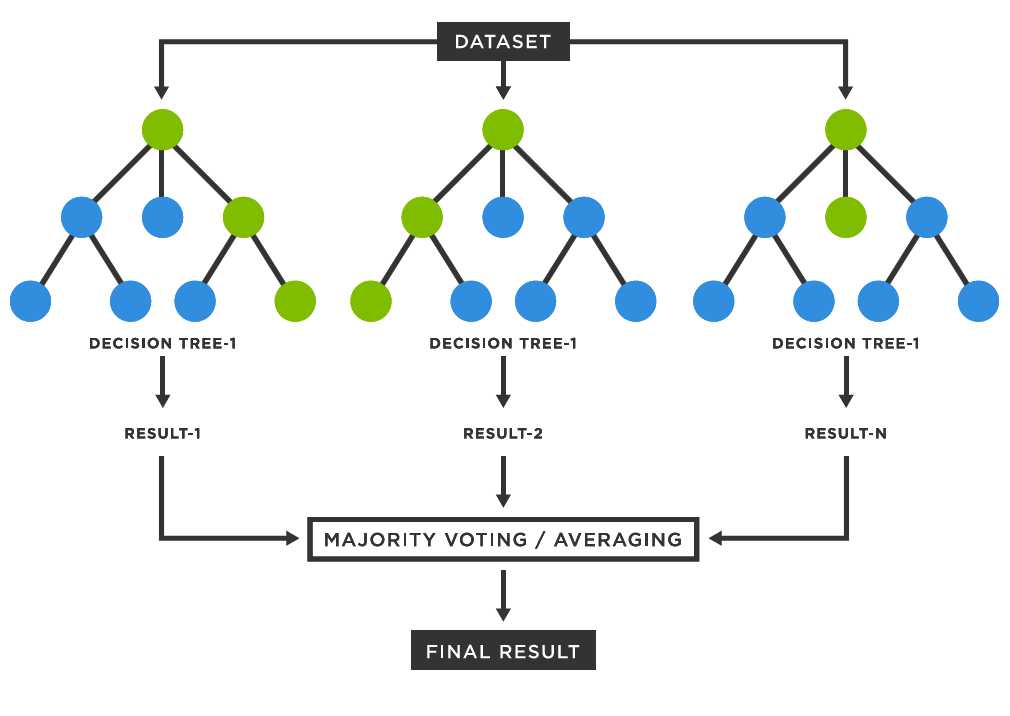
\includegraphics[scale=0.4]{LaTeX Bachelor Thesis Depression Signs Detection/figures/RandomForestVisualized.png}
        \caption{Random Forest Visualized \cite{predikdata2023}}
	\label{randomForestVisualized}
\end{figure}

One of the key features of Random Forest is that it introduces randomness not only in the selection of data samples but also in the selection of features used to split nodes in the trees. This randomness helps in making the model less likely to overfit the training data. Overfitting occurs when a model learns the training data too well, including its noise and outliers, and performs poorly on new, unseen data.

In classification tasks, each decision tree in the forest votes for a class, and the class with the most votes is chosen as the final prediction. In regression tasks, the average of the outputs from all trees is taken as the final result. This ensemble approach generally leads to higher accuracy and better generalization compared to using a single decision tree.

Random Forest has several advantages. It is easy to use and tune, often requiring fewer parameters compared to other complex algorithms. It handles large datasets with higher dimensionality well and maintains good performance even when a large proportion of the data is missing. Additionally, it can give insights into the importance of different features in the data, which can be useful for understanding underlying patterns.

However, Random Forest also has some limitations. It can be computationally expensive and slow to train when dealing with a large number of trees or very large datasets. The model can also become less interpretable as the number of trees increases, making it harder to understand the decision-making process compared to a single decision tree.

\section{Evaluation Metrics}
\quad Metrics are a crucial part of evaluating the effectiveness of a binary classifier. It's important to use a variety of tools and methods to understand different aspects of the model's performance. Here the metrics that were chosen for the evaluation of the depression binary classifier:

\begin{itemize}
     \item \textbf{Confusion Matrix}: This is a table that visualizes the performance of the binary classifier by showing the actual versus predicted classifications. The matrix contains the values: TP (true positives), TN (true negatives), FP (false positives), and FN (false negatives). It helps identify the kinds of errors the model is making, such as confusing one class for another.
     
    \item \textbf{Classification Metrics}: These include accuracy, precision, recall, and the F1-score, which together provide a comprehensive overview of overall model performance. 
    \begin{itemize}
        \item \textbf{Accuracy} measures the overall correctness of the model across all predictions (formula \ref{accuracy}). 
        \item \textbf{Precision} assesses how many of the positively predicted cases were actually positive 
 (formula \ref{precision}).
        \item \textbf{Recall} (or sensitivity) determines how many of the actual positive cases were correctly identified by the model (formula \ref{recall}).
        \item \textbf{F1-Score} is the harmonic mean of precision and recall, helping balance the two in scenarios where one may be more important than the other 
 (formula \ref{f1}).
        
        \begin{align} 
            &\mathit{Accuracy} = \frac{TP+TN}{TP+TN+FP+FN} \label{accuracy}\\
            &\mathit{Precision} = \frac{TP}{TP+FP} \label{precision}\\
            &\mathit{Recall} = \frac{TP}{TP+FN} \label{recall}\\
            &F1-Score = \frac{2*\mathit{Precision}*\mathit{Recall}}{\mathit{Precision}+\mathit{Recall} \label{f1}}
        \end{align}
    \end{itemize}
       \item \textbf{ROC Curve}: This graph shows the ability of the model to distinguish between the two classes at various threshold levels. It plots the true positive rate against the false positive rate, providing insight into the trade-offs between capturing positives and avoiding false alarms \cite{hoo2017roc}.
    \item \textbf{Feature Importance}: This metric highlights which features (variables) in your data have the most influence on the model’s predictions. Understanding feature importance can help in refining the model by focusing on the most relevant factors.
\end{itemize}

By using these metrics, a detailed understanding of your model's strengths and weaknesses can be achieved, guiding improvements and ensuring it performs well across various conditions.